\section{Optimizer and Learning Rate Scheduling}



We use Adam Optimizer with the defauls settings given in \verb|torch.optim.Adam| documentation \href{https://pytorch.org/docs/stable/generated/torch.optim.Adam.html}{here}.
\begin{verbatim}
    betas = (0.9 , 0.999)
    eps = 1e-08
    weight_decay = 0
\end{verbatim}

For \verb|scheduling| the \verb|learning rate|, we use \verb|torch.optim.lr_scheduler.CosineAnnealingLR| with settings,

For the first $80$ \verb|epochs|, we start with \verb|learning rate| $10^{-3}$, ending to $5 \times 10^{-4}$ and use,
\begin{verbatim}
    T_max = 160
    eta_min = 0
    last_epoch = -1
\end{verbatim}

For the next $180$ \verb|epochs|, we start with \verb|learning rate| $3 \times 10^{-4}$ and use,
\begin{verbatim}
    T_max = 160
    eta_min = 0
    last_epoch = -1
\end{verbatim}

The jump in the \verb|Learning Rate| in \autoref{fig:part1_lr} is hence explained.
 

\begin{figure}[htbp]
  \centering
  \begin{minipage}[b]{0.45\textwidth}
    \centering
    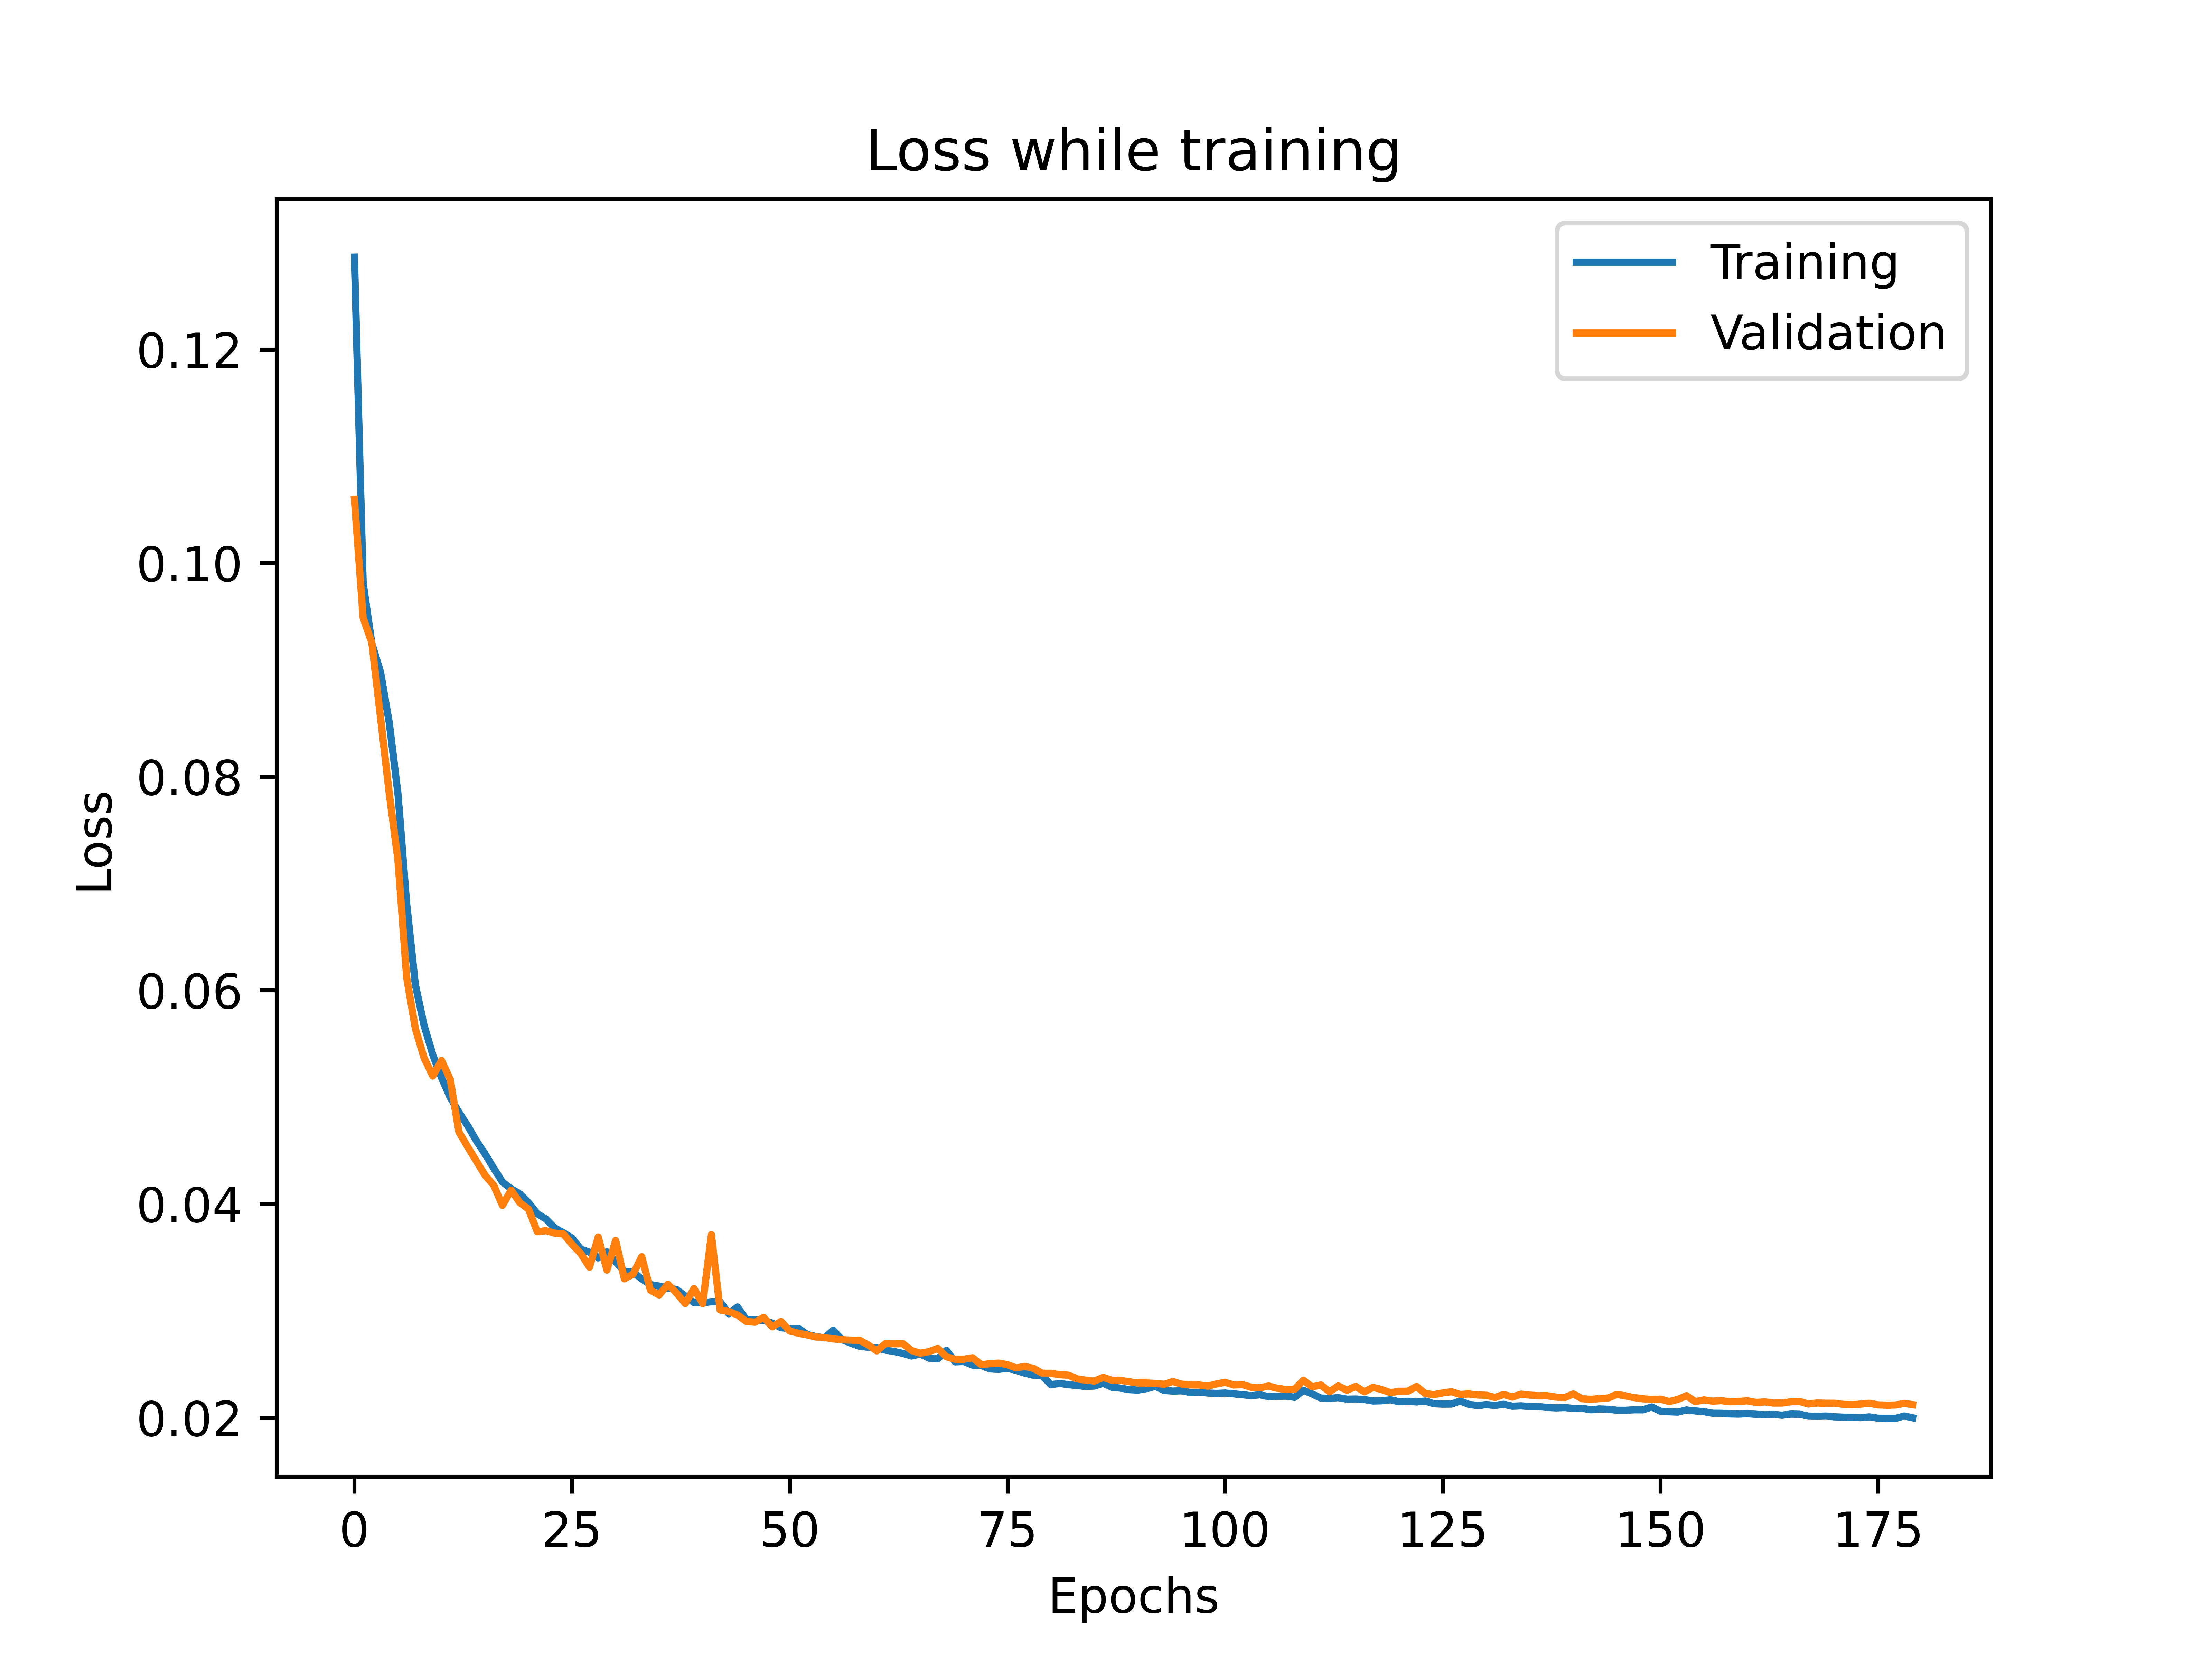
\includegraphics[width=\textwidth]{images/loss_curves_part1.png}
    \caption{Loss curves}
    \label{fig:part1_loss}
  \end{minipage}
  \hfill
  \begin{minipage}[b]{0.45\textwidth}
    \centering
    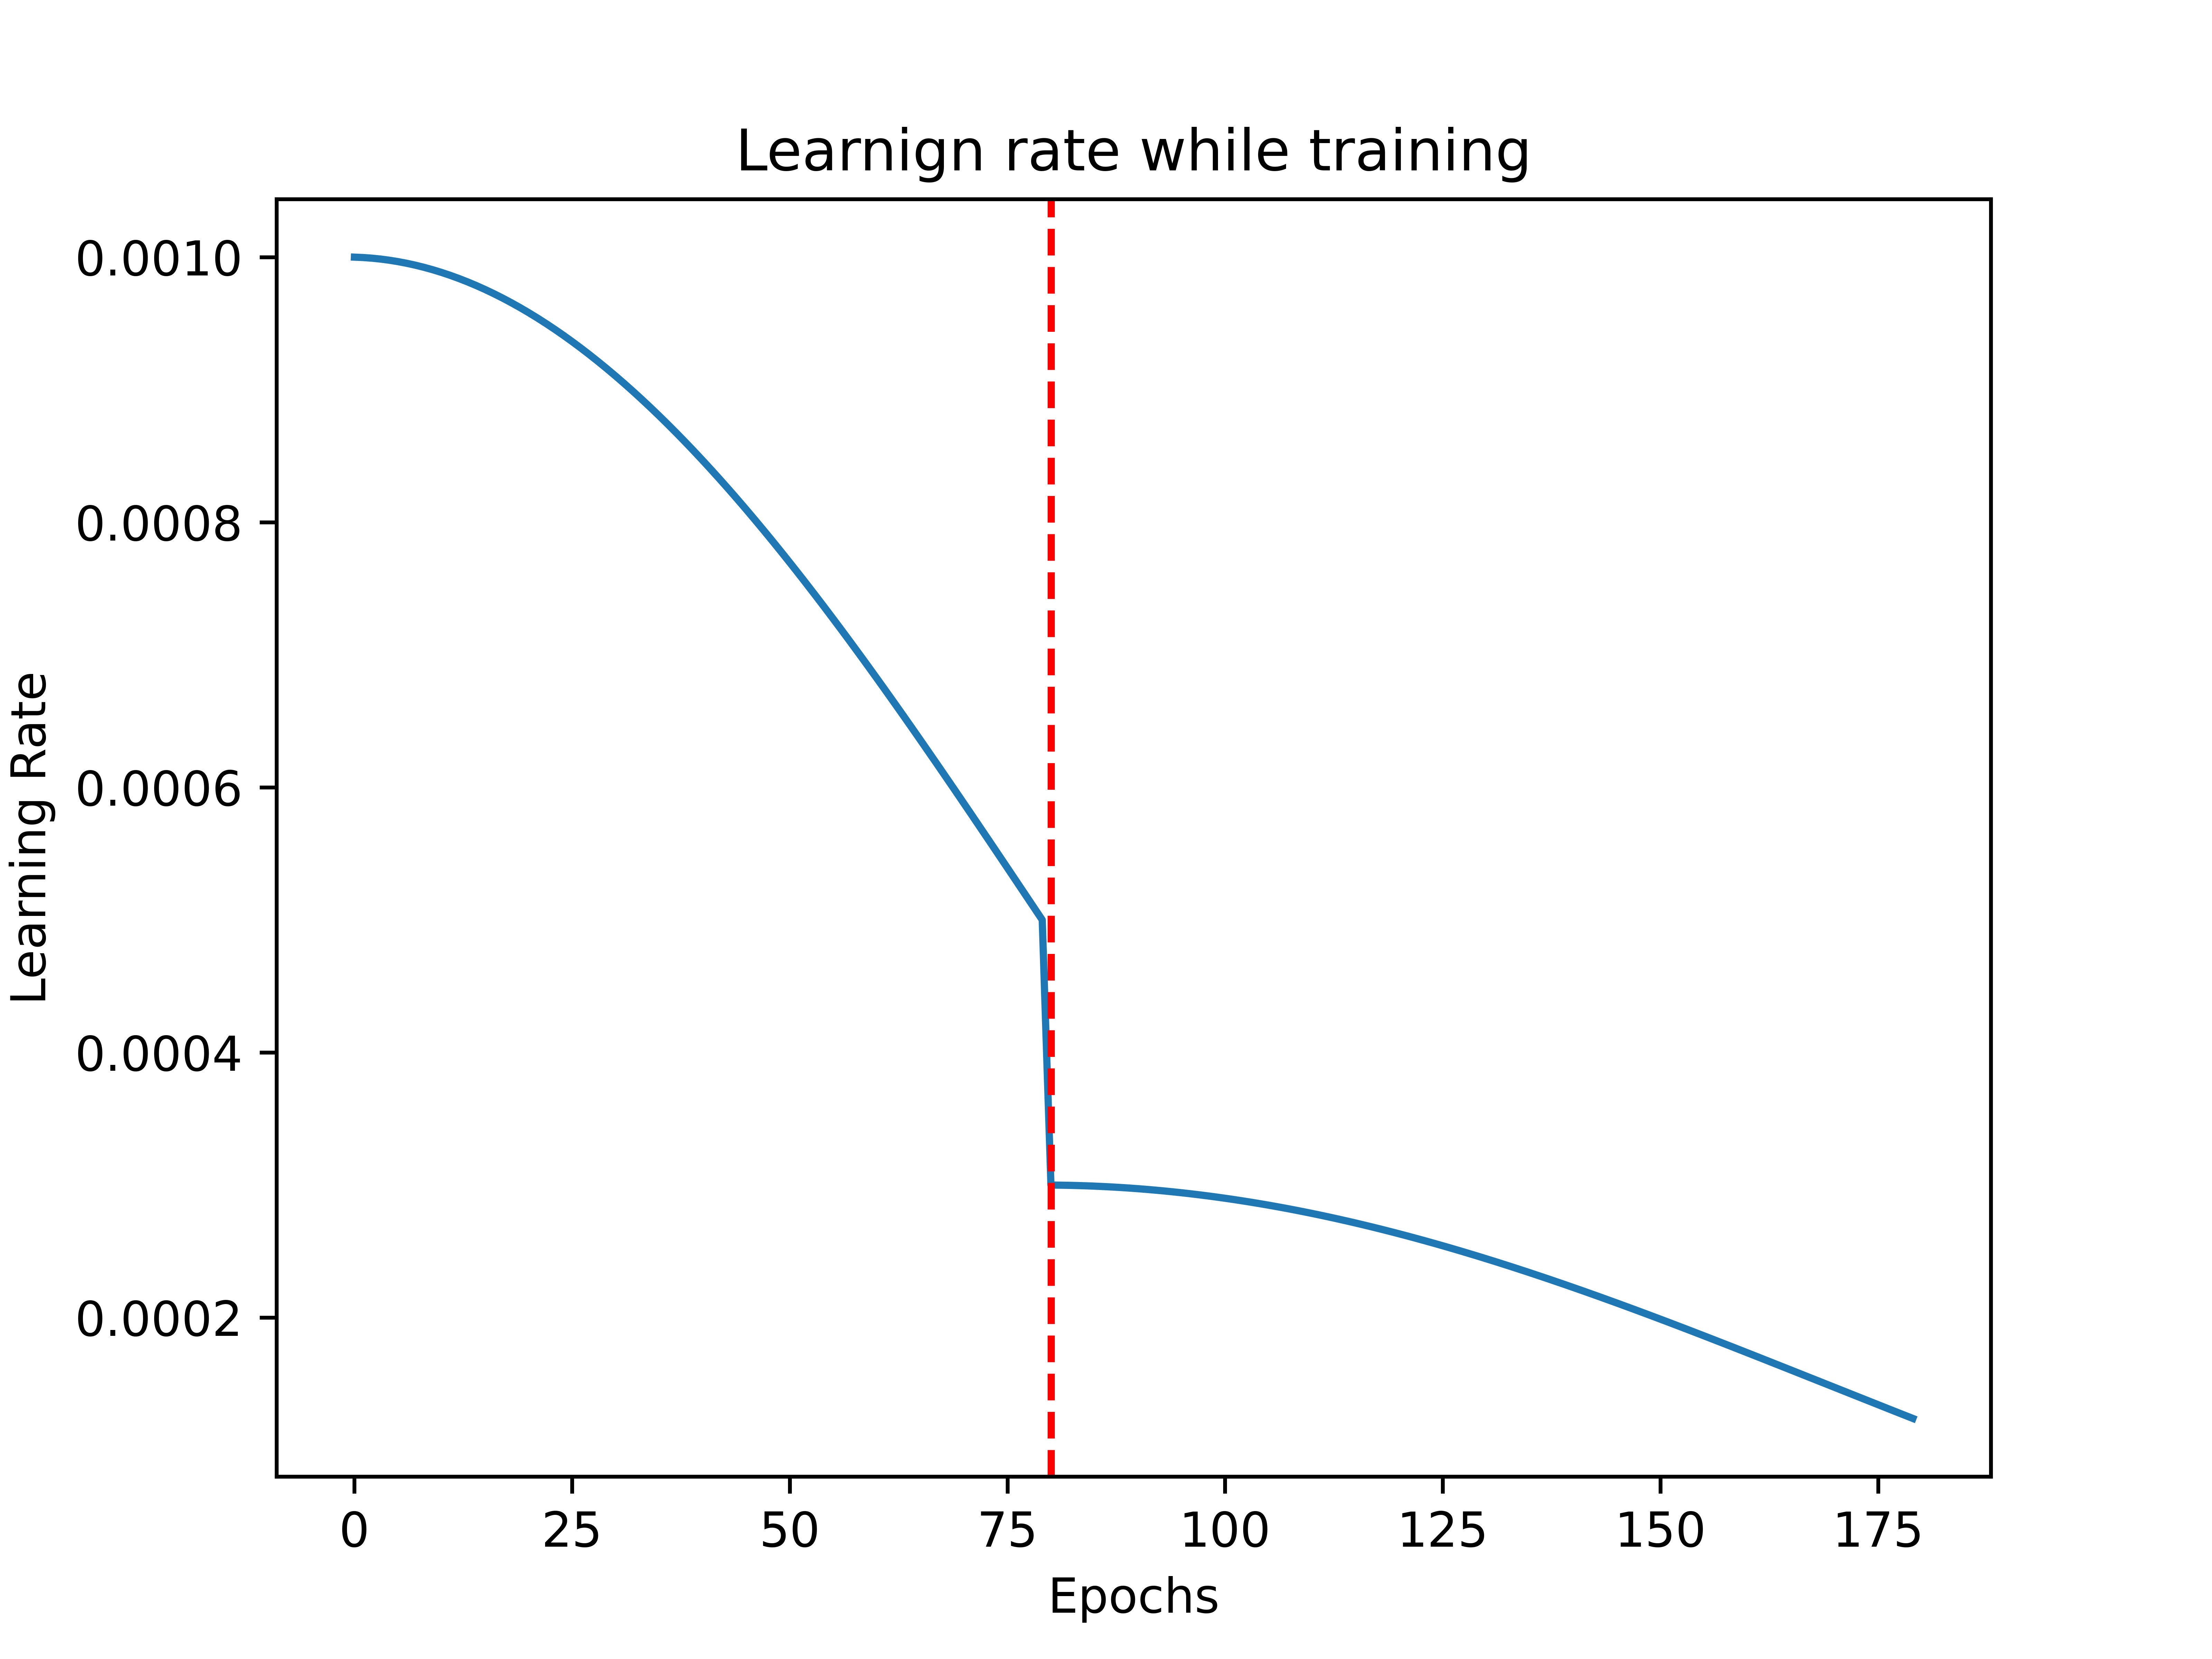
\includegraphics[width=\textwidth]{images/learning_rate_part1.png}
    \caption{Learning Rate}
    \label{fig:part1_lr}
  \end{minipage}
  \caption{Slot Attention model}
\end{figure}


